\documentclass{ximera}

\author{Anna Davis} \title{MTH 160 Homework 2} 

\begin{document}

\begin{abstract}

\end{abstract}
\maketitle
 \textit{Certificate due: 9/1/2021 at 11:59 p.m.}
 \section{Lecture 2}
\begin{problem}\label{prob:160hom2prob1}
Find the domain of each function and express it in interval notation.  (Hint: type the word "infinity" to get the $\infty$ symbol.)
\begin{enumerate}
    \item $f(x)=\frac{1}{x^2}$
    $$\answer{(-\infty,0)}\cup\answer{(0,\infty)}$$
    \item $f(x)=\frac{1}{x^2-1}$
    $$\answer{(-\infty,-1)}\cup\answer{(-1,1)}\cup\answer{(1,\infty)}$$
    \item $f(x)=\frac{1}{x^2+1}$
    $$\answer{(-\infty,\infty)}$$
    \item $f(x)=\sqrt{2x-4}$
    $$\answer{[2,\infty)}$$
     \item $f(x)=\frac{1}{\sqrt{x-3}}$
    $$\answer{(3,\infty)}$$
    \item $f(x)=\frac{x+1}{(x-4)(x+7)}$
    $$\answer{(-\infty,-7)}\cup\answer{(-7,4)}\cup\answer{(4,\infty)}$$
\end{enumerate}
\end{problem}

\begin{problem}\label{prob:160hom2prob2}
  Find the range of each function and express it in interval notation.  (Hint: type the word "infinity" to get the $\infty$ symbol.)
  \begin{enumerate}
      \item $f(x)=x^2+2$
      $$\answer{[2,\infty)}$$
      \item $f(x)=-x^2$
      $$\answer{(-\infty,0]}$$
  \end{enumerate}
\end{problem}

\begin{problem}\label{prob:160hom2prob3}
Find the domain and range for each function represented graphically.
\begin{enumerate}
    \item Graph of f:
     \begin{image}
   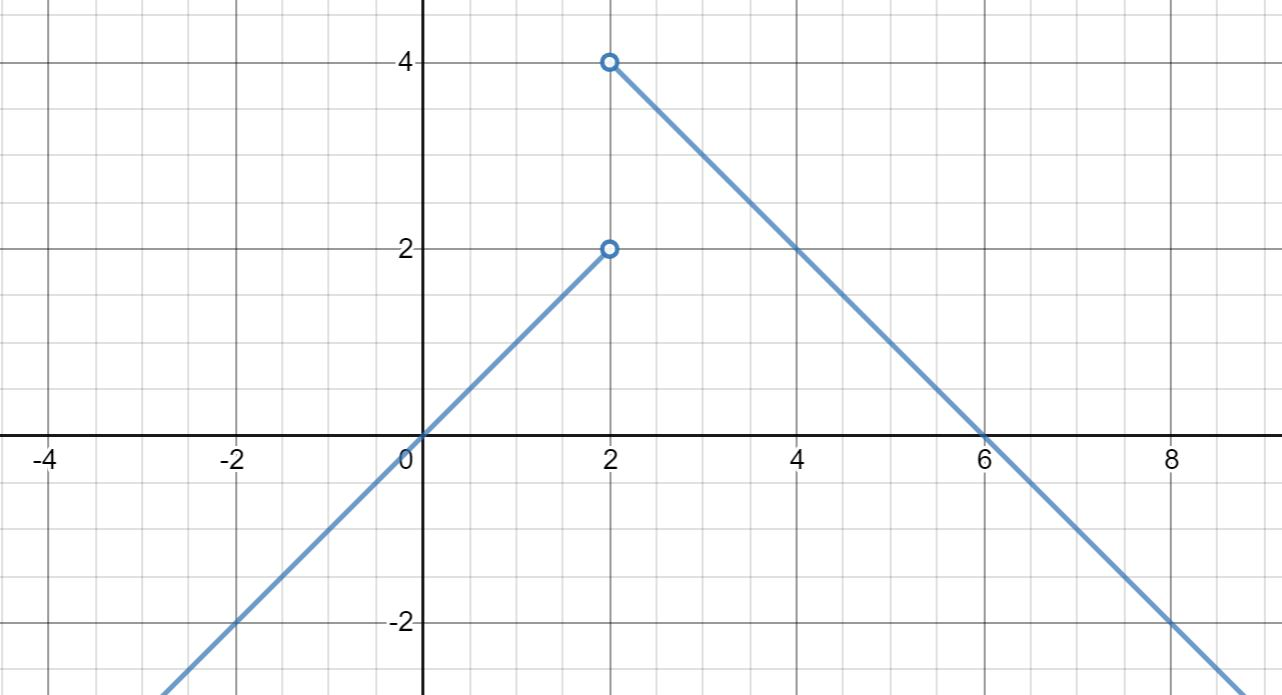
\includegraphics[height=1in]{160H2pic1.jpg}
 \end{image}
 
 Domain: $\answer{(-\infty,2)}\cup\answer{(2,\infty)}$
 
 Range:  $\answer{(-\infty,4)}$
 \item Graph of f:
     \begin{image}
   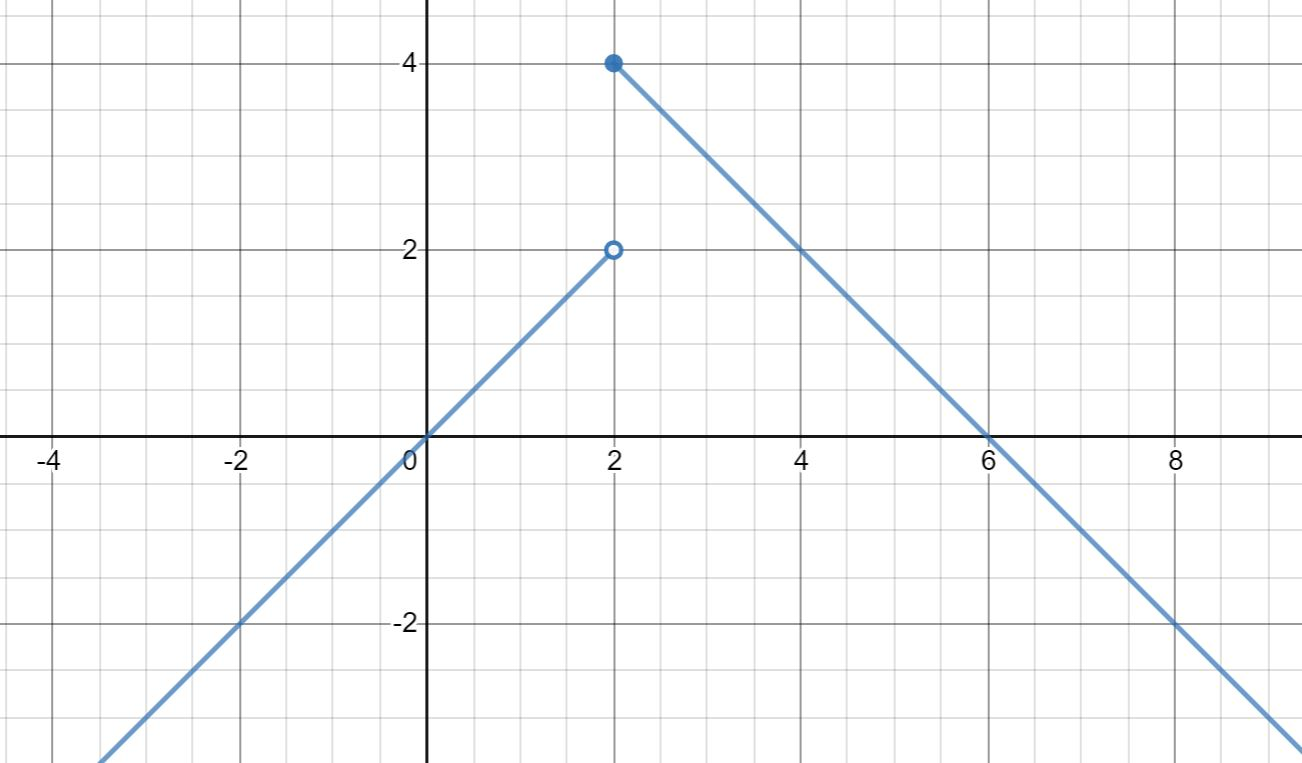
\includegraphics[height=1in]{160H2pic2.jpg}
 \end{image}
 
 Domain:$\answer{(-\infty,\infty)}$
 
 Range:  $\answer{(-\infty,4]}$
 \item Graph of f:
     \begin{image}
   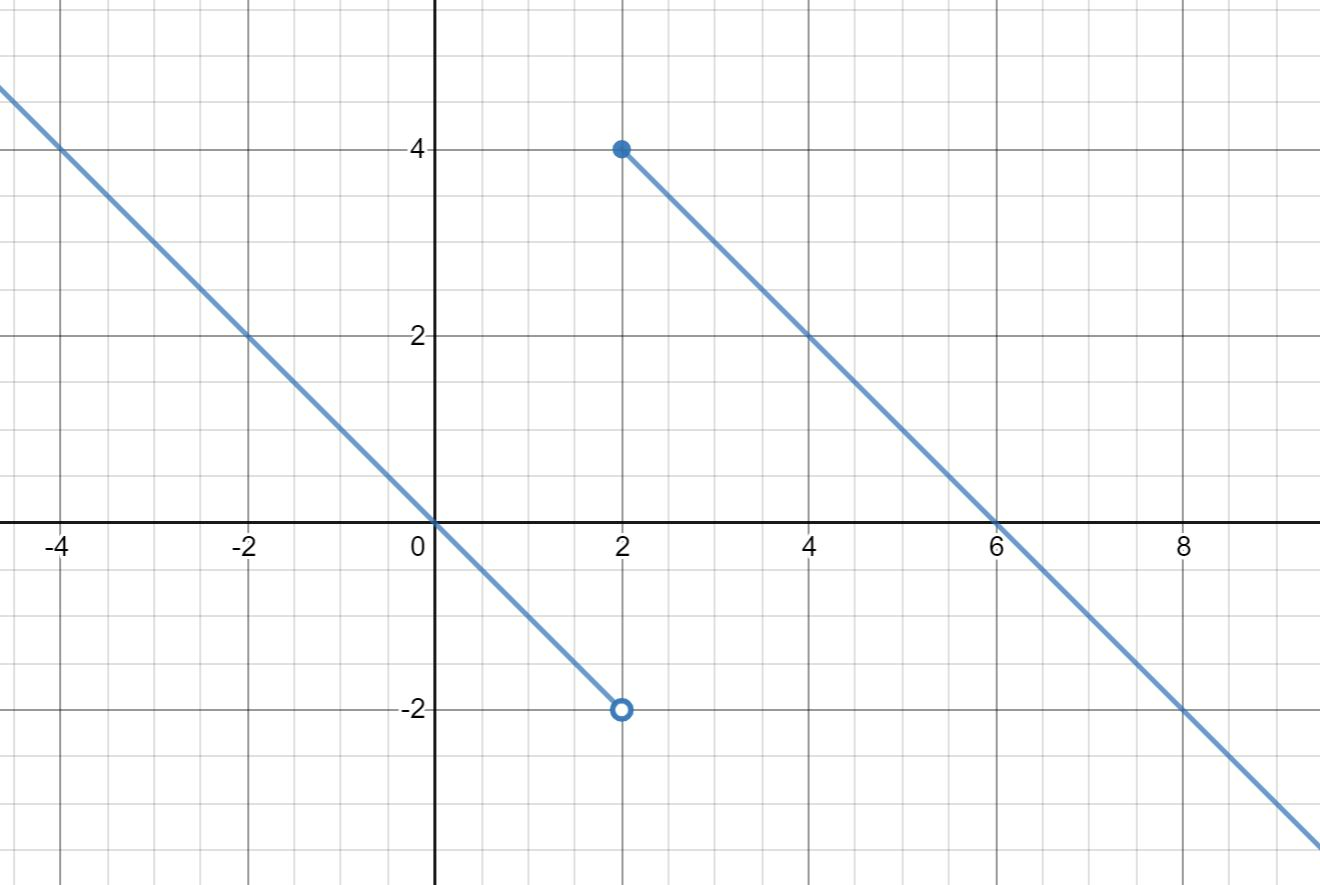
\includegraphics[height=1in]{160H2pic3.jpg}
 \end{image}
 
 Domain: $\answer{(-\infty,\infty)}$
 
 Range: $\answer{(-\infty,\infty)}$
 \item Graph of f:
     \begin{image}
   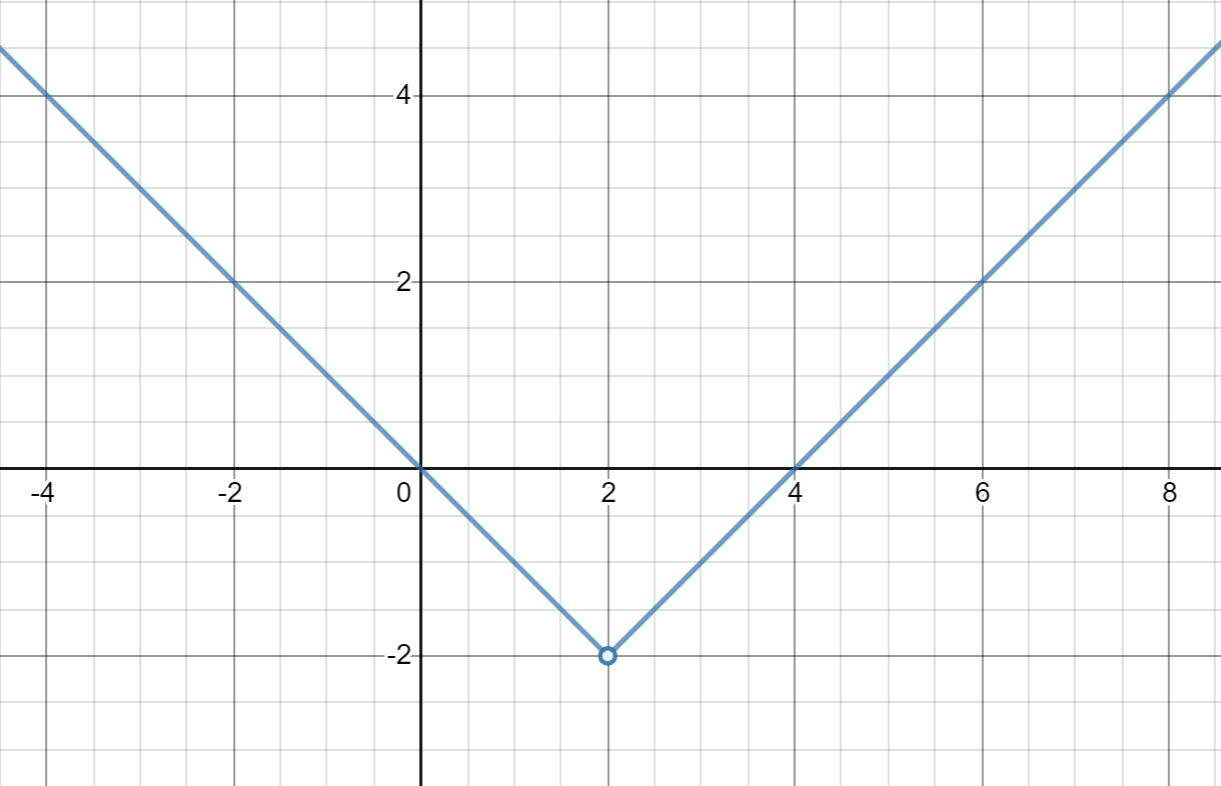
\includegraphics[height=1in]{160H2pic4.jpg}
 \end{image}
 
 Domain:  $\answer{(-\infty,2)}\cup\answer{(2,\infty)}$
 
 Range: $\answer{(-2,\infty)}$
 \item Graph of f:
     \begin{image}
   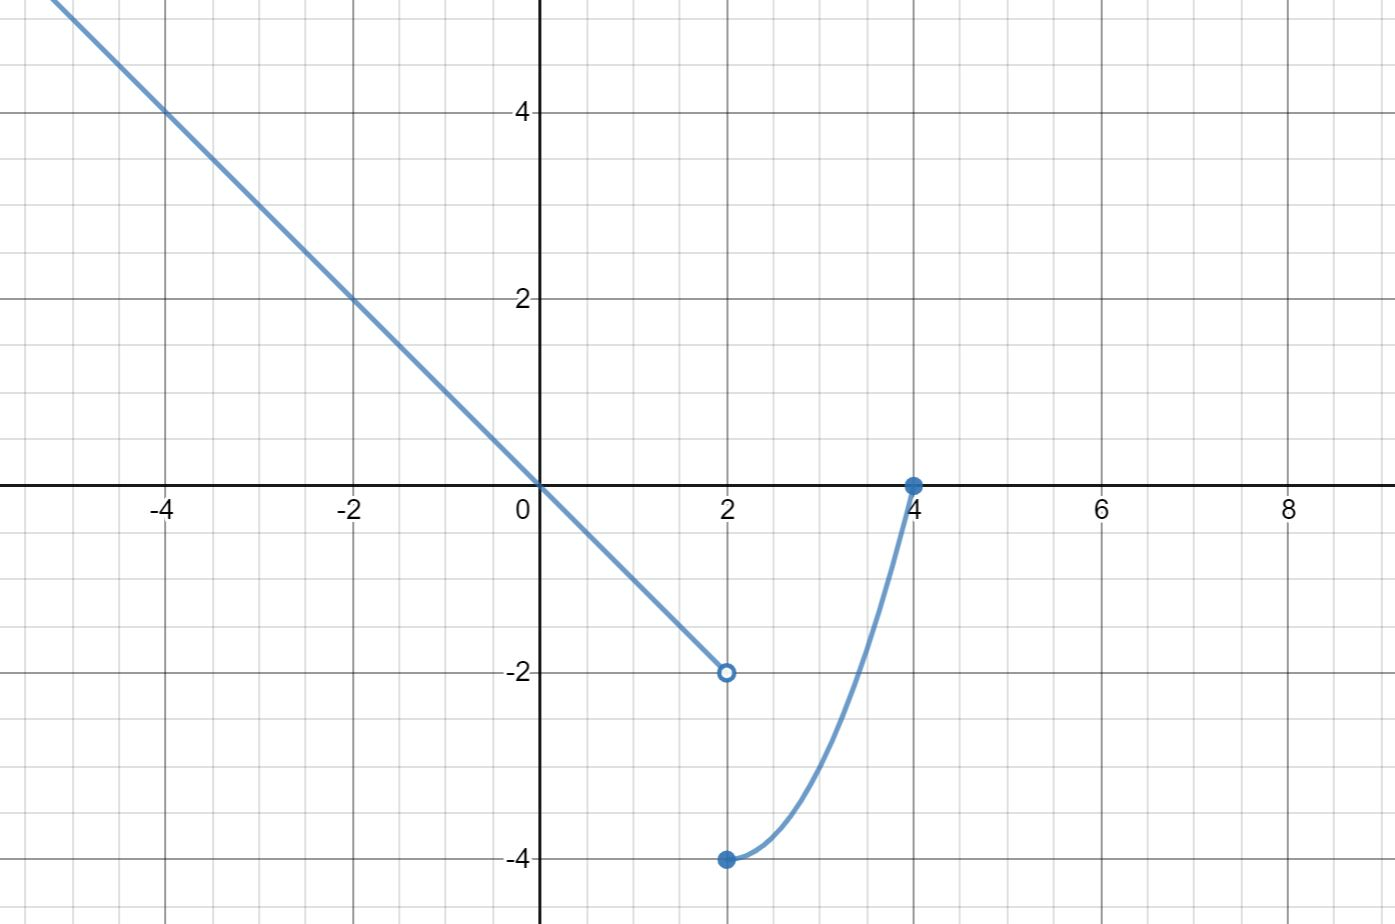
\includegraphics[height=1in]{160H2pic5.jpg}
 \end{image}
 
 Domain: $\answer{(-\infty,4]}$
 
 Range: $\answer{[-4,\infty)}$
\end{enumerate}
\end{problem}
\section{Lecture 3}
\begin{problem}\label{prob:160hom2prob4}
Select the function that best matches the given graph.
\begin{image}
   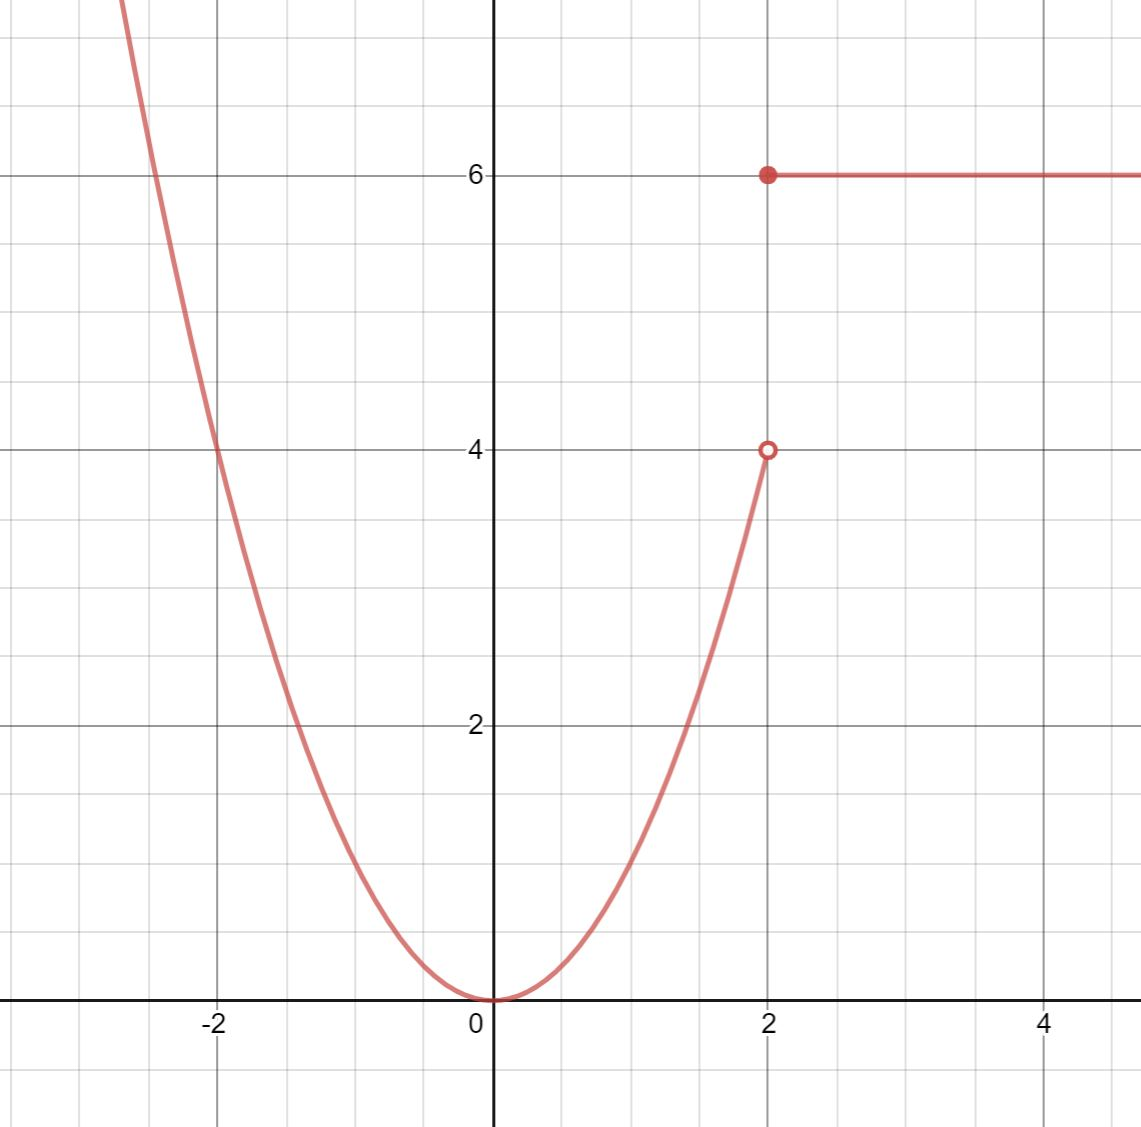
\includegraphics[height=1in]{160H2pic6.jpg}
 \end{image}
\begin{multipleChoice}  
\choice{$g(x)= \begin{cases} 
      x^2 & x\leq 4 \\
      \frac{1}{x} & x>6 
   \end{cases}
$}  
\choice{$g(x)= \begin{cases} 
      x^2 & x\leq 2 \\
      6 & x>2 
   \end{cases}
$}  
\choice{$g(x)= \begin{cases} 
      6 & x\leq 2 \\
      x^2 & x>2 
   \end{cases}
$}  
\choice[correct]{$g(x)= \begin{cases} 
      x^2 & x< 2 \\
      6 & x\geq 2 
   \end{cases}
$}  
\end{multipleChoice}  
\end{problem}

\begin{problem}\label{prob:160hom2prob5}
Select the function that best matches the given graph.
\begin{image}
   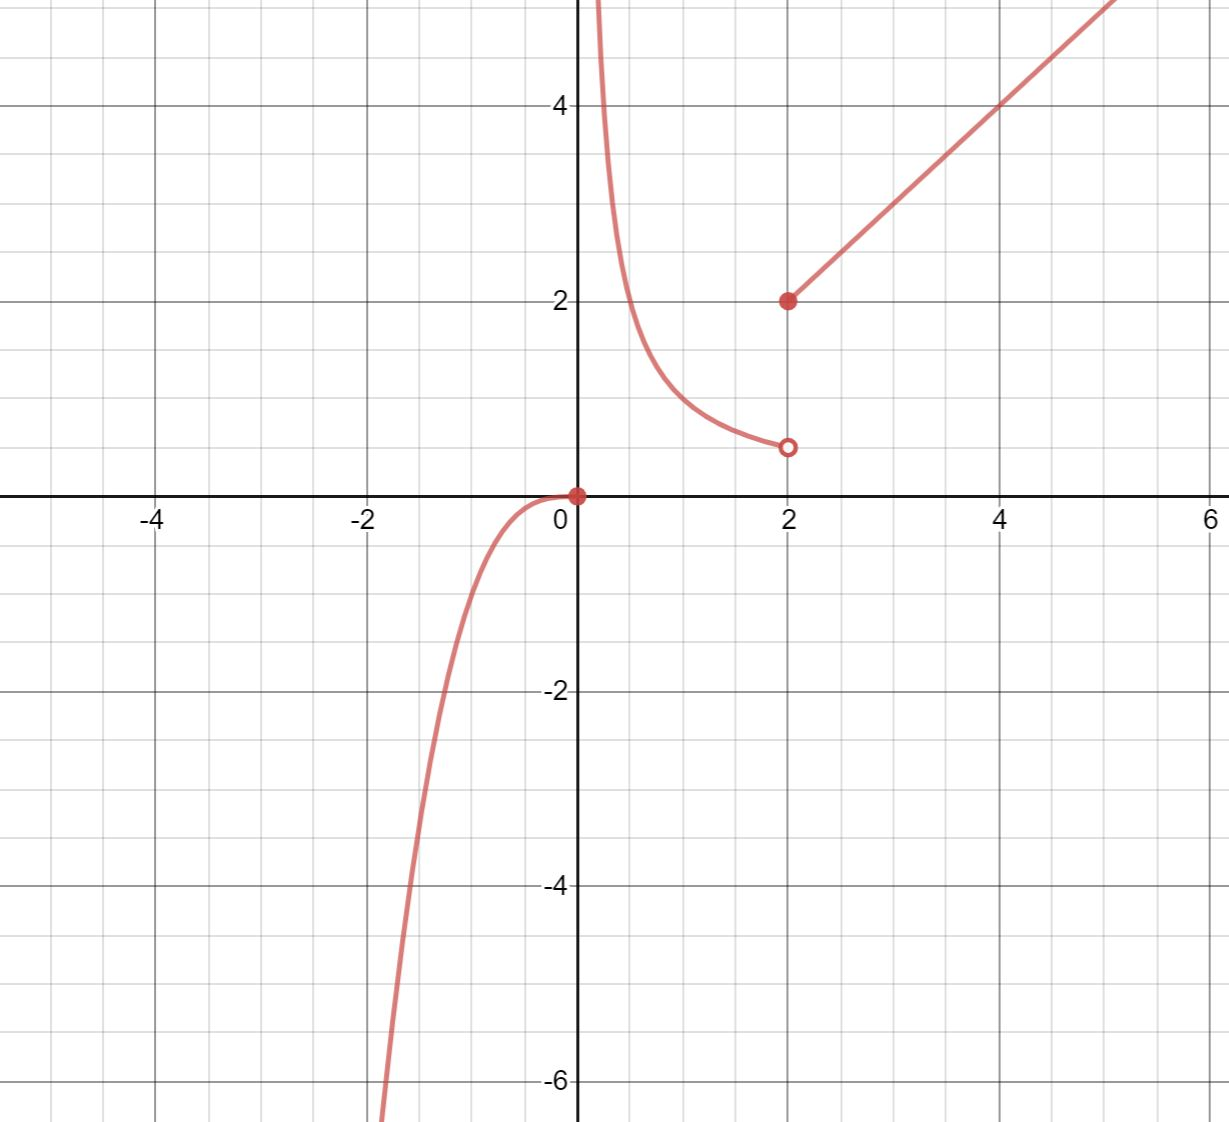
\includegraphics[height=1in]{160H2pic7.jpg}
 \end{image}
\begin{multipleChoice}  
\choice[correct]{$g(x)= \begin{cases} 
      x^3 & x\leq 0 \\
      \frac{1}{x} & 0<x<2\\
      x& x\geq 2
   \end{cases}
$}  
\choice{$g(x)= \begin{cases} 
      -x^2 & x\leq 0 \\
      \frac{1}{x} & 0<x<2\\
      x& x\geq 2
   \end{cases}
$}  
\choice{$g(x)= \begin{cases} 
      x^3 & x<0 \\
      \frac{1}{x} & 0<x<1/2\\
      x& x\geq 2
   \end{cases}
$}  
\choice{$g(x)= \begin{cases} 
      x^3 & x< 0 \\
      \frac{1}{x} & 0\leq x<2\\
      x& x\geq 2
   \end{cases}
$}  
\end{multipleChoice}  

\end{problem}
\section{Lecture 4}
\begin{problem}\label{prob:160hom2prob6}
Let $f(x)=2x^2-x$ and $g(x)=-x^2+3$.  Evaluate each expression.
\begin{enumerate}
    \item $(f\circ g)(0)=\answer{15}$
    \item $(f\circ g)(2)=\answer{3}$
    \item $(f\circ g)(-3)=\answer{78}$
    \item $(g\circ f)(0)=\answer{3}$
    \item $(g\circ f)(-1)=\answer{-6}$
    \item $(f\circ f)(2)=\answer{66}$
    \item $(g\circ g)(-2)=\answer{2}$
\end{enumerate}
\end{problem}

\begin{problem}\label{prob:160hom2prob7}
The graphs of $f$ and $g$ are shown.  Use the graphs to evaluate each expression.
\begin{image}
   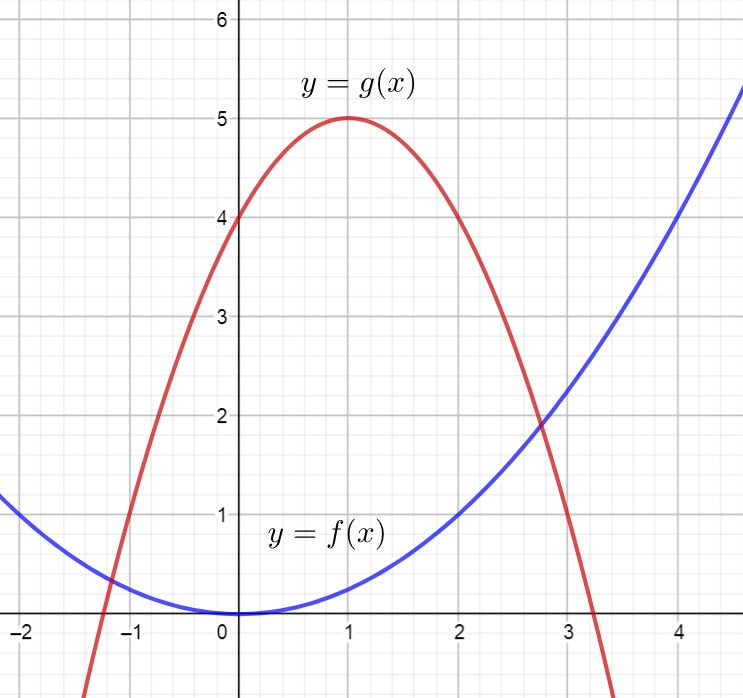
\includegraphics[height=1in]{160H2pic8.jpg}
 \end{image}
  \begin{enumerate}
\item
$(g\circ f)(2)=\answer{5}$

\item
$(f\circ g)(0)=\answer{4}$

  \end{enumerate}
\end{problem}
\begin{problem}\label{prob:160hom2prob8}
Let $f(x)=-3x^2-2x+1$ and $g(x)=4x-1$.  Evaluate each expression and simplify as much as possible.
\begin{enumerate}
    \item $(g\circ f)(x)=\answer{-12}x^2-\answer{8}x+\answer{3}$
    \item $(f\circ g)(x)=\answer{-48}x^2+\answer{16}x$
    \item $(g\circ g)(x)=\answer{16x-5}$ (Enter symbolic expression containing $x$.)
\end{enumerate}
\end{problem}
\end{document} 